\section{Topologia: Computação como uma mercadoria}

O conceito da nuvem é construído sobre camadas, cada uma fornecendo um nível 
distinto de funcionalidade~\cite{cloud-computing-fundamentals}. Essa estratificação 
dos componentes forneceu o meio para que as camadas da computação em nuvem se 
tornassem uma mercadoria, como eletricidade, serviço telefônico ou gás natural. A 
mercadoria que a computação em nuvem vende é poder computacional a um custo e 
despesas menores para o usuário. Espera-se que a computação em nuvem se torne o 
próximo serviço megautilitário~\cite{cloud-computing-fundamentals}.

Como exemplo, explicaremos o \emph{Virtual Machine Monitor} (VMM) da IBM. Ele 
fornece o meio para uso simultâneo das instalações de nuvem (figura \ref{fig:vmm}). 
VMM é um programa em um sistema host que permite que um computador suporte diversos 
ambientes de execução idênticos~\cite{cloud-computing-fundamentals}. Do ponto de 
vista do usuário, o sistema é um computador autocontido que é isolado dos outros 
usuários. Na realidade, cada usuário está sendo servido pela mesma máquina. Na 
computação em nuvem, o VMM permite que usuários monitorem e gerenciem aspectos do 
processo, tais como acesso a dados, armazenamento de dados, criptografia, 
endereçamento, topologia e movimento de carga de 
trabalho~\cite{cloud-computing-fundamentals}. 


\begin{figure}[ht]
    \centering
    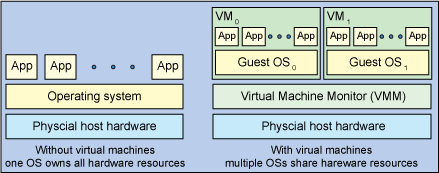
\includegraphics[width=0.6\textwidth]{img/vmm.png}
    \caption{Como o Virtual Machine Monitor
        funciona~\cite{cloud-computing-fundamentals}.
    } 
    \label{fig:vmm}
\end{figure}


As camadas principais que a nuvem oferece são~\cite{cloud-computing-fundamentals}:

\newcommand{\itemm}[1]{\item\textbf{#1}}

\begin{itemise}

    \itemm{IaaS --- Infrastructure as a Service:} Camada que constitui a base da 
    nuvem. Consiste nos ativos físicos --- servidores, dispositivos de rede, discos 
    de armazenamento, etc. Ao usar IaaS, o cliente não controla de fato a 
    infraestrutura subjacente, mas sim os sistemas operacionais, armazenamento, 
    aplicativos de implementação e, até certo ponto, os componentes de rede 
    selecionados. 

    Serviços de \emph{Print On Demand} (POD) são um exemplo de organizações que 
    podem se beneficiar da IaaS. O modelo de POD é baseado na venda de produtos 
    customizados, onde pessoas podem abrir lojas e vender designs de produtos. Os 
    lojistas podem carregar o número de designs que quiserem à medida que os criam. 
    Muitos carregam milhares. Com recursos de armazenamento em nuvem, um POD pode 
    fornecer espaço de armazenamento ilimitado.

    \itemm{PaaS --- Plataform as a Service:} Camada intermediária. Fornece acesso a 
    sistemas operacionais e serviços associados, além de uma maneira de implementar 
    aplicativos para a nuvem usando linguagens de programação e ferramentas 
    suportadas pelo fornecedor. Não é necessário gerenciar ou controlar a 
    infraestrutura subjacente; o cliente tem controle dos aplicativos implementados 
    e, até certo ponto, de configurações de ambiente de \emph{hosting} de 
    aplicativos. 

    PaaS tem provedores como \emph{Elastic Compute Cloud} (EC2) da Amazon. A pequena 
empresa de software é um empreendimento ideal para PaaS. Com a plataforma elaborada,
produtos de classe mundial podem ser criados sem o gasto adicional da produção
interna.

    \itemm{SaaS --- Software as a Service:} É a camada superior (a de aplicativo), a 
    qual a maioria visualiza como a nuvem. Aplicativos são executados aqui e são 
    fornecidos sob demanda para os usuários. SaaS tem provedores como \emph{Google 
    Pack}, que inclui aplicativos que podem ser acessados pela Internet, ferramentas 
    como Gmail, Google Talk, Docs e outros.

\end{itemise}

\begin{figure}[H]
    \centering
    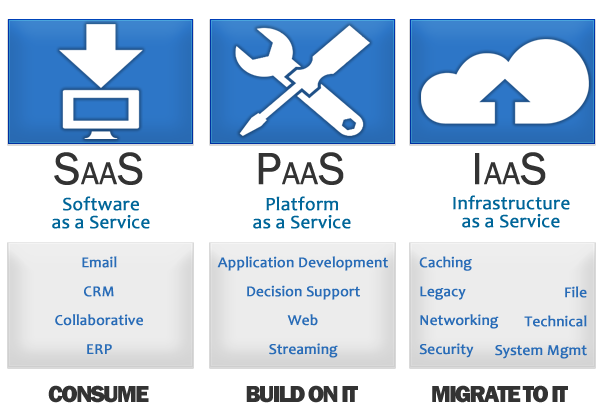
\includegraphics[width=0.5\textwidth]{img/services2.png}
    \caption{Principais camadas de computação em nuvem integradas nos componentes
        "como serviço"~\cite{code-trick-getting-started-cloud}}
    \label{fig:layers}
\end{figure}


Existem também outros serviços oferecidos pela computação em 
nuvem~\cite{informatica}:

\begin{itemise}

    \itemm{DevaaS - Development as a Service:} As ferramentas de desenvolvimento 
    tomam forma na computação em nuvem como ferramentas compartilhadas, ferramentas 
    de desenvolvimento \emph{web-based} e serviços baseados em \emph{mashup}. 

    \itemm{CaaS - Communication as a Service:} Uso de uma solução de comunicação 
    unificada hospedada em data center do provedor ou fabricante (exemplo: Microsoft 
    Lync). 

    \itemm{EaaS - Everything as a Service:} Quando tudo é utilizado: infraestrurura, 
    plataformas, software, suporte... Enfim, o que envolve Tecnologia da Informação 
    e Comunicação como um serviço. 

    \itemm{DBaas - Database as a Service:} Quando a parte de servidores de banco de 
    dados é utilizada como serviço.

    \itemm{TaaS - Testing as a Service:}: Oferece um ambiente apropriado para que o 
    usuário possa testar aplicações e sistemas de maneira remota, simulando o 
    comportamento destes em nível de execução.

\end{itemise}

\undef\itemm

% \begin{figure}[ht]
%     \centering
%     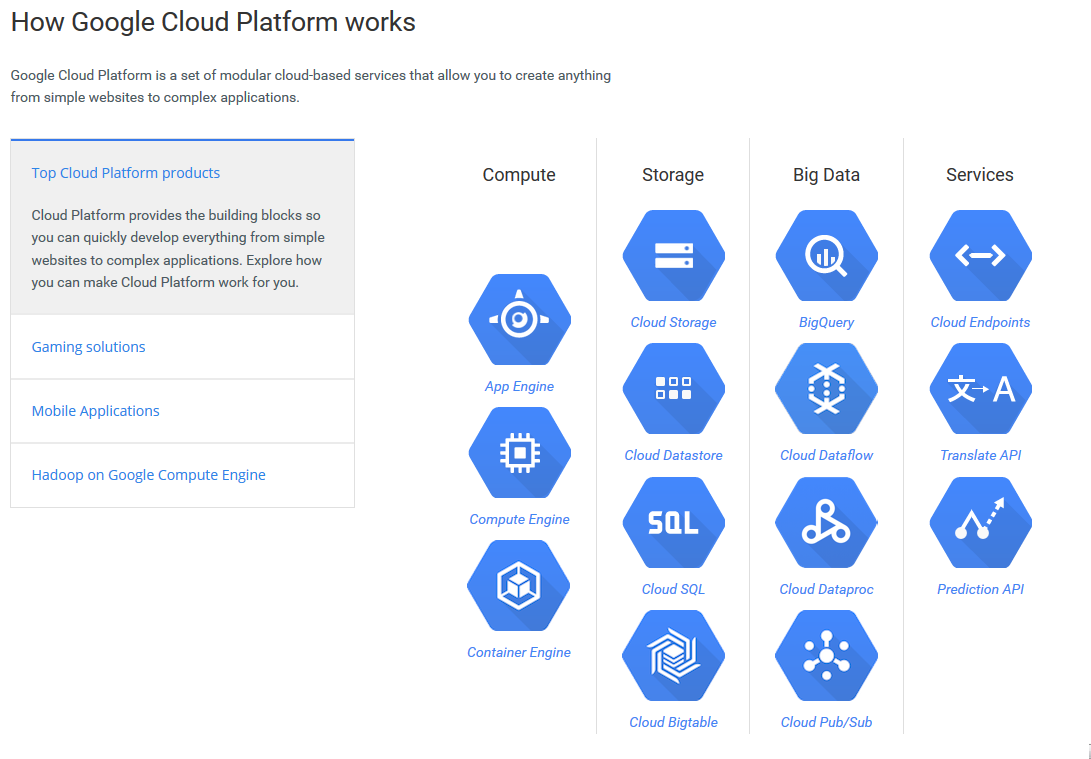
\includegraphics[width=0.8\textwidth]{img/googlecloud.png}
%     \caption{Exemplo do provedor
%              \href{https://cloud.google.com/}{Google~Cloud~Platform}
%              para os serviços oferecidos para computação em nuvem
%             }
%     \label{img:googlecloud}
% \end{figure}
